\chapter{Progettazione della base di dati}\label{cha:progdbasdata}
\minitoc\mtcskip

\textsc{Allegato}: viene fornito il modello del database \texttt{database/DATABASE.sql}

In questo documento procederemo ad effettuare le seguenti analisi:
\begin{itemize}
\diam \textit{Progettazione del Database tramite modello ER}: (v. Sezione 
	\vref{sec:projdata}) identificheremo la struttura logica del nostro 
	database, per poi effettuare la traduzione in linguaggio SQL3
	
\diam \textit{Analisi del Framework}: (v. Sezione \vref{sec:dbutilizzejp}) ci preoccupiamo 
	di come di effettuare il mapping dei dati memorizzati all'interno di un 
	database relazionale, in un linguaggio Object Oriented.
\end{itemize}

\section{Analisi dei requisiti}\label{sec:projdata}
Questa coincide con l'analisi del Piano di Sviluppo presentata nel Capitolo
\vref{cha:pds}. Possiamo sottolineare che la realizzazione di una base di 
dati all'interno del nostro progetto sia necessaria, in quanto è necessario 
mantenere dei dati persistenti all'interno della nostra applicazione.

\section{Progettazione concettuale}
Dal modello di dominio, possiamo ottenere un modello equivalente per la nostra
base di dati, che può essere tradotto in un diagramma \textsc{Entity-Relationship}\footnote{
NOTA: all'interno dei diagrammi ER, per ogni entità si descrive «\textit{il numero
minimo e massimo di occorrenze di relazione, a cui una occorrenza dell'entità 
può partecipare}» (Atzeni, Ceri, Paraboschi, Torlone: ``\textit{Basi di dati: Modelli
e linguaggi di interrogazione''}. McGraw-Hill Edizioni.)} (d'ora in poi ER).
Contestualmente ampliamo il Glossario della Sezione \vref{sec:glossario} con 
il Glossario dei dati in Tabella \vref{tab:ddd}, dove indichiamo per ciascuna 
entità gli attributi corrispondenti; non palesiamo inoltre il significato 
delle relazioni, in quanto di per se deducibili nella Figura \vref{fig:seed}.

\begin{table}[p]

\begin{tabularx}{\columnwidth}{XXXX}
\toprule
Entità & Descrizione & Attributi & Id\\
\midrule
\textbf{Tutore} & \textit{Ha la supervisione del minorenne e vi accede in sua vece}.
	& Nome, Cognome, Indirizzo, Numero di telefono, E-Mail, Data di nascita,
	Password & \textsc{Codice fiscale}\\
\textbf{Paziente minorenne} & \textit{Necessita della mediazione di un tutore per accedere
	al sistema}. &  & \\
\textbf{Paziente maggiorenne} & \textit{Può accedere ed interagire col sistema senza la 
	mediazione di un tutore}. &  & \\
\textbf{Paziente} & \textit{Astrazione di un generico cliente che può ricevere delle cure} & 
	Nome, Cognome, Indirizzo, Numero di telefono, E-Mail, 
	Data di nascita, Password & \textsc{Codice fiscale}\\ 
\textbf{Referto} & \textit{Fornisce il responso dei medici in seguito alla visita del
	paziente} & \textsc{Id} &\\
\textbf{Prenotazione} & \textit{Indica quando un paziente potrà accedere alle cure} & 
	Priorità, Medico, Ora, Data & \textsc{Id}\\
\textbf{Amministratore} & \textit{Può gestire le prenotazioni del sistema attinenti al
	suo reparto} & & \textsc{Nome utente, Password}\\
\textbf{Reparto} & \textit{Identifica le tipologie di visite che possono essere 
	effettuate all'interno delle sue sale} & & \textsc{Nome}\\
\textbf{Sala} & \textit{Identifica il luogo dove possono avvenire le visite di un tale
	reparto}. & & \textsc{Numero}\\
\end{tabularx}
\bigskip


\caption{\textit{Dizionario dei Dati}.}\label{tab:ddd}
\end {table}

\begin{figure}[!t]
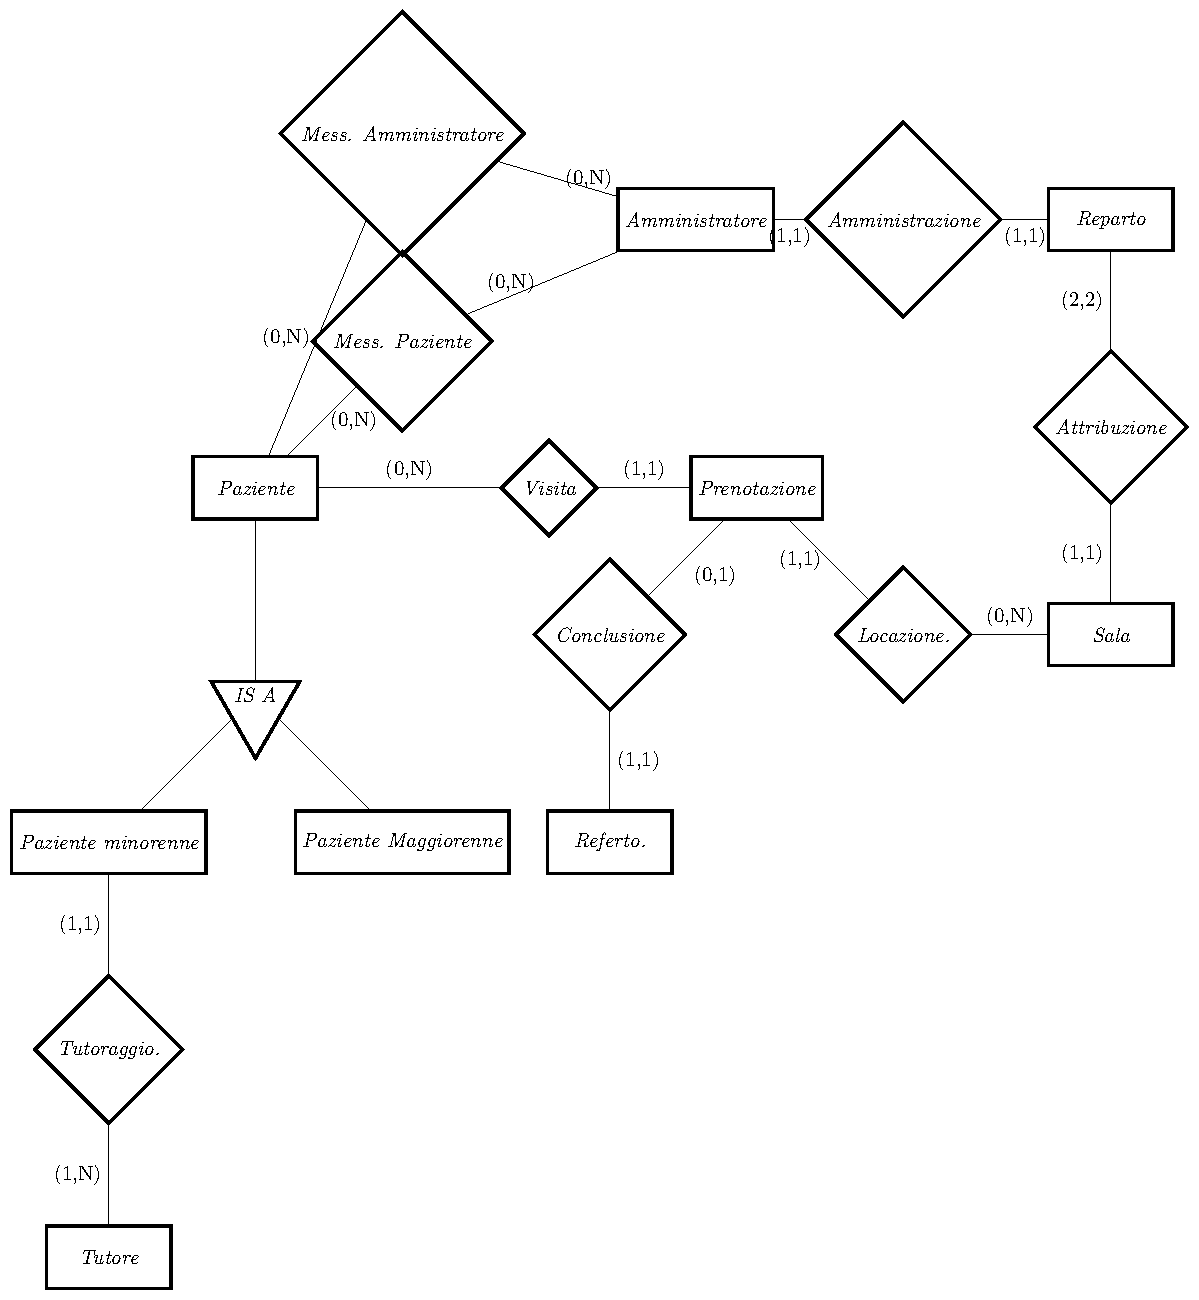
\includegraphics[scale=0.8]{er2/first}
\caption{\textit{First ER diagram}.}
\label{fig:seed}
\end{figure}

\section{Progettazione Logica}\label{sec:proglogicadb}
Dall'analisi dei requisiti non funzionali del nostro sistema, posiamo ottenere 
la Tavola dei Volumi e delle Operazioni osservabile in Tabella \vref{tab:tdvedo}.
I valori di cui sotto ci sono stati forniti dal cliente come stima per eccesso
dei dati della clinica di un anno.


\begin{table}[!t]
\begin{tabular}{lcc}
\toprule
Nome & Tipo & Volume \\
\midrule
\textbf{Tutore} & E & 15\\
\textbf{Paziente minorenne} & E & 30\\
\textbf{Paziente maggiorenne} & E & 42\\
\textbf{Paziente} & E & 72\\
\textbf{Referto} & E & 135\\
\textbf{Prenotazione} & E & 225\\
\textbf{Amministratore} & E & 2\\
\textbf{Reparto} & E & 2\\
\textbf{Sala} & E & 4\\
\textbf{Tutoraggio} & R & 45\\
\textbf{Mess. Paziente} & R & 230\\
\textbf{Mess. Amministratore} & R & 230\\
\textbf{Visita} & R & 230\\
\textbf{Amministrazione} & R & 2\\
\textbf{Attribuzione} & R & 4\\
\textbf{Locazione} & R & 225\\
\textbf{Conclusione} & R & 135\\
\end{tabular}
\caption{\textit{Tavola dei Volumi e delle Operazioni}.}
\label{tab:tdvedo}
\end{table}

\subsection{Eliminazione delle generalizzazioni}
In quanto la soluzione di ``accorpamento del genitore nelle generalizzazioni
figlie'' comporti il dover periodicamente verificare se gli utenti minorenni 
abbiano o meno raggiunto la maggiore età, andando quindi ad aumentare il numero
delle operazioni non necessarie all'interno del database, si ritiene utile
effettuare un ``accorpamento delle entità figlie nella generalizzazione del
genitore''. Ciò risulta altresì vantaggioso in quanto le entità figlie possono
essere distinte dalla presenza o meno della relazione con il Tutore, che è inoltre
l'unica per la quale l'entità figlia Paziente Minorenne distingue l'entità 
Paziente Maggiorenne. Conseguentemente, all'interno della Base di Dati, potremmo
ottenere un'unica entità Paziente. 

Inoltre, in quanto è presente una relazione (1-1) tra amministratore e reparto,
possiamo ipotizzare un'unione tra le due tabelle, andando ad identificare ciascun
amministratore con un reparto di pertinenza. Si rivela però necessario aggiungere
un attributo di \textsc{Reparto}.

Il risultato ottenuto è il diagramma rappresentato in Figura \vref{fig:feed}.

\begin{figure}[!t]
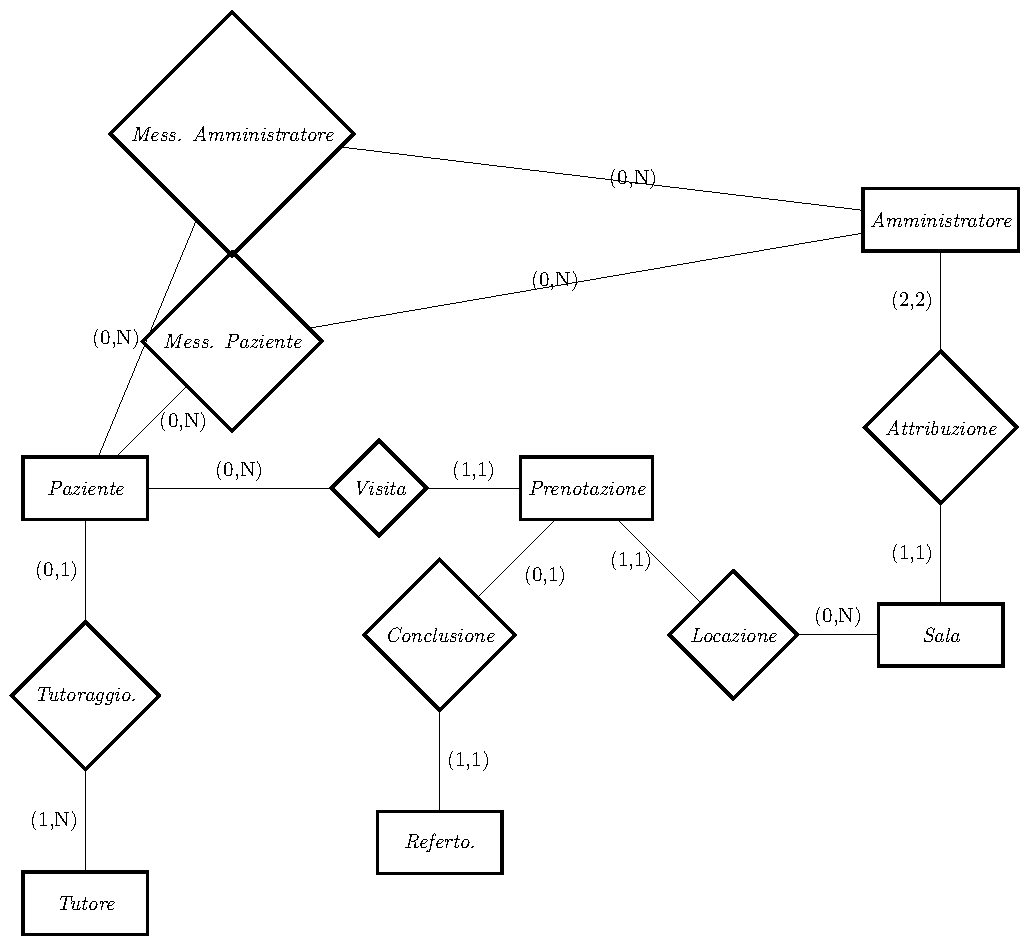
\includegraphics[scale=0.8]{er2/second}
\caption{\textit{Final ER diagram}.}
\label{fig:feed}
\end{figure}

\section{Traduzione Logica}
Traduciamo il diagramma in relazioni.
\begin{description}

\item[Amministratore] 
\begin{center}
\texttt{
Amministratore(\uline{NomeUtente}, Password)
}
\end{center}

\item[Referto] 
\begin{center}
\texttt{
Referto(\uline{Id}, Contenuto)
}
\end{center}

\item[Sala] 
\begin{center}
\texttt{
Sala(\uline{Numero}, Amministratore)
}
\end{center}

\item[Tutore] 
\begin{center}
\texttt{
Tutore(\uline{CF}, Nome, Cognome, Indirizzo, Numero di telefono, E-Mail, Data di nascita,
	Password)
}
\end{center}

\item[Paziente] Identifichiamo il Paziente Maggiorenne da quello Minorenne dalla
	presenza o meno del tutore.
\begin{center}
\texttt{
Paziente(\uline{CF}, Nome, Cognome, Indirizzo, Numero di telefono, E-Mail, Data di nascita,
	Password, Tutore)
}
\end{center}

\item[Prenotazione] 
\medskip

\begin{center}
\texttt{
Prenotazione(\uline{Id}, Priorità, Medico, Ora, Data, Referto, Sala)
}
\end{center}

\item[Messaggi Paziente] 
\begin{center}
\texttt{
MPaziente(\uline{Paziente}, \uline{Amministratore})
}
\end{center}

\item[Messaggi Amministratore] 
\begin{center}
\texttt{
MAmministratore(\uline{Amministratore}, \uline{Paziente})
}
\end{center}

\end{description}

Forniamo quindi di seguito il listato del database:

\lstinputlisting[language=SQL]{database/DATABASE.sql}

\section{Installazione del database}
Si consiglia di installare il software \textsc{PostgreSQL} per la gestione del
database: per creare un nuovo database per un utente che vi ha i privilegi di
accesso, digitare:
\begin{center}
\texttt{createdb orthopediatrics}
\end{center}


dove \texttt{orthopediatrics} è il nome del database. Per importare il database
dal file \texttt{database/DATABASE.sql} digitare:
\begin{center}
\texttt{cat database/DATABASE.sql | psql -d orthopediatrics}
\end{center}

\section{Utilizzo del Framework EJP}\label{sec:dbutilizzejp} 
Abbiamo scelto di utilizzare il \textit{framework} ``Easy Java Persistence''\footnote{
\texttt{http://www.easierjava.com}} in quanto semplificava notevolmente il processo
di interfacciamento con il database, in quanto non sono necessarie nè configurazioni
tramite file XML, nè si ha la necessità di estendere classi o di implementare
interfacce fornite dal nostro framework.  

Altro vantaggio di questo framework è dovuto al fatto che modifiche al database,
non implicano dirette modifiche agli oggetti del nostro applicativo e viceversa:
predispone inoltre di metodi di \textit{rollback} e la definizione di \textit{transactions}
per non rendere inconsistente lo stato del nostro database.

Parallelamente, è necessario effettuare alcuni accorgimenti all'interno della
definizione delle nostre classi:
\begin{itemize}
\item La definizione di una classe \texttt{Classname} è elemento sufficiente per
	accedere alla tabella \texttt{classname} del nostro database.
\item È opportuno definire degli attributi che corrispondano agli attributi delle
	tabelle, contemporaneamente a dei metodi \textit{getter} e \textit{setter}.
\item È opportuno definire per ogni classe un metodo \texttt{toString()}.
\item Ogni relazione con una tabella \texttt{Foreign} è mappata all'interno della
	classe come una \texttt{List<Foreign>}.
\end{itemize}

In questo modo si rivela non necessaria la definizione di un servizio di 
comunicazione \textit{client-server}, in quanto già questo framework supporta
meccanismi di sincronizzazione e di accesso remoto ai database.
